\documentclass[aspectratio=169]{beamer}
\usetheme{Madrid}
\usecolortheme{default}

\usepackage{booktabs}
\usepackage{graphicx}
\usepackage{array}

\title[Pythia-160M Seed-9 Alignment]{Pythia-160M Seed-9 Alignment Transfer}
\subtitle{Repeat-match causal head roles across all official seeds}
\author{Branch specialization research project}
\date{2026-05-22}

\begin{document}

\begin{frame}
  \titlepage
  \vspace{-0.5em}
  \small
  Checkpoint reason: this is the full 9-seed replication of the Pythia-160M
  repeat-match alignment-transfer result.
\end{frame}

\begin{frame}{Question}
  The 3-seed Pythia-160M run suggested that raw-score alignment transfers
  repeat-match causal head roles much better than same head index.

  \vspace{0.8em}
  This checkpoint asks:

  \vspace{0.5em}
  \begin{center}
  \textit{does that aligned-transfer result survive all 9 official Pythia-160M
  seeds?}
  \end{center}

  \vspace{0.8em}
  This is the current strongest test of weak, relabeled cross-seed role
  universality in the project.
\end{frame}

\begin{frame}{Setup}
  \begin{itemize}
    \item Models: \texttt{EleutherAI/pythia-160m-seed1} through seed9
    \item Checkpoints: step4000, step16000, step143000
    \item Layers: 0 and 1
    \item Selected heads: top repeat-match head per tested layer
    \item Alignment: raw attention-score Hungarian matching using all 8 fixed
    probe texts
    \item Causal test: zero selected head outputs; measure repeated-token
    continuation loss
    \item Transfer pairs: 72 ordered source-target seed pairs per checkpoint
  \end{itemize}
\end{frame}

\begin{frame}{Metric Glossary}
  \begin{description}
    \item[Probe specialization] Normalized repeat-match attention pattern score.
    \item[Own top minus random] Target seed selected-head loss delta minus random
    same-layer controls.
    \item[Same-index transfer] Ablate target seed heads at the source seed's raw
    layer/head indices.
    \item[Aligned transfer] Ablate target seed heads matched to source heads by
    raw-score alignment.
    \item[Aligned better] Number of source-target pairs where aligned transfer
    has larger loss delta than same-index transfer.
  \end{description}
\end{frame}

\begin{frame}{Trajectory}
  \begin{center}
    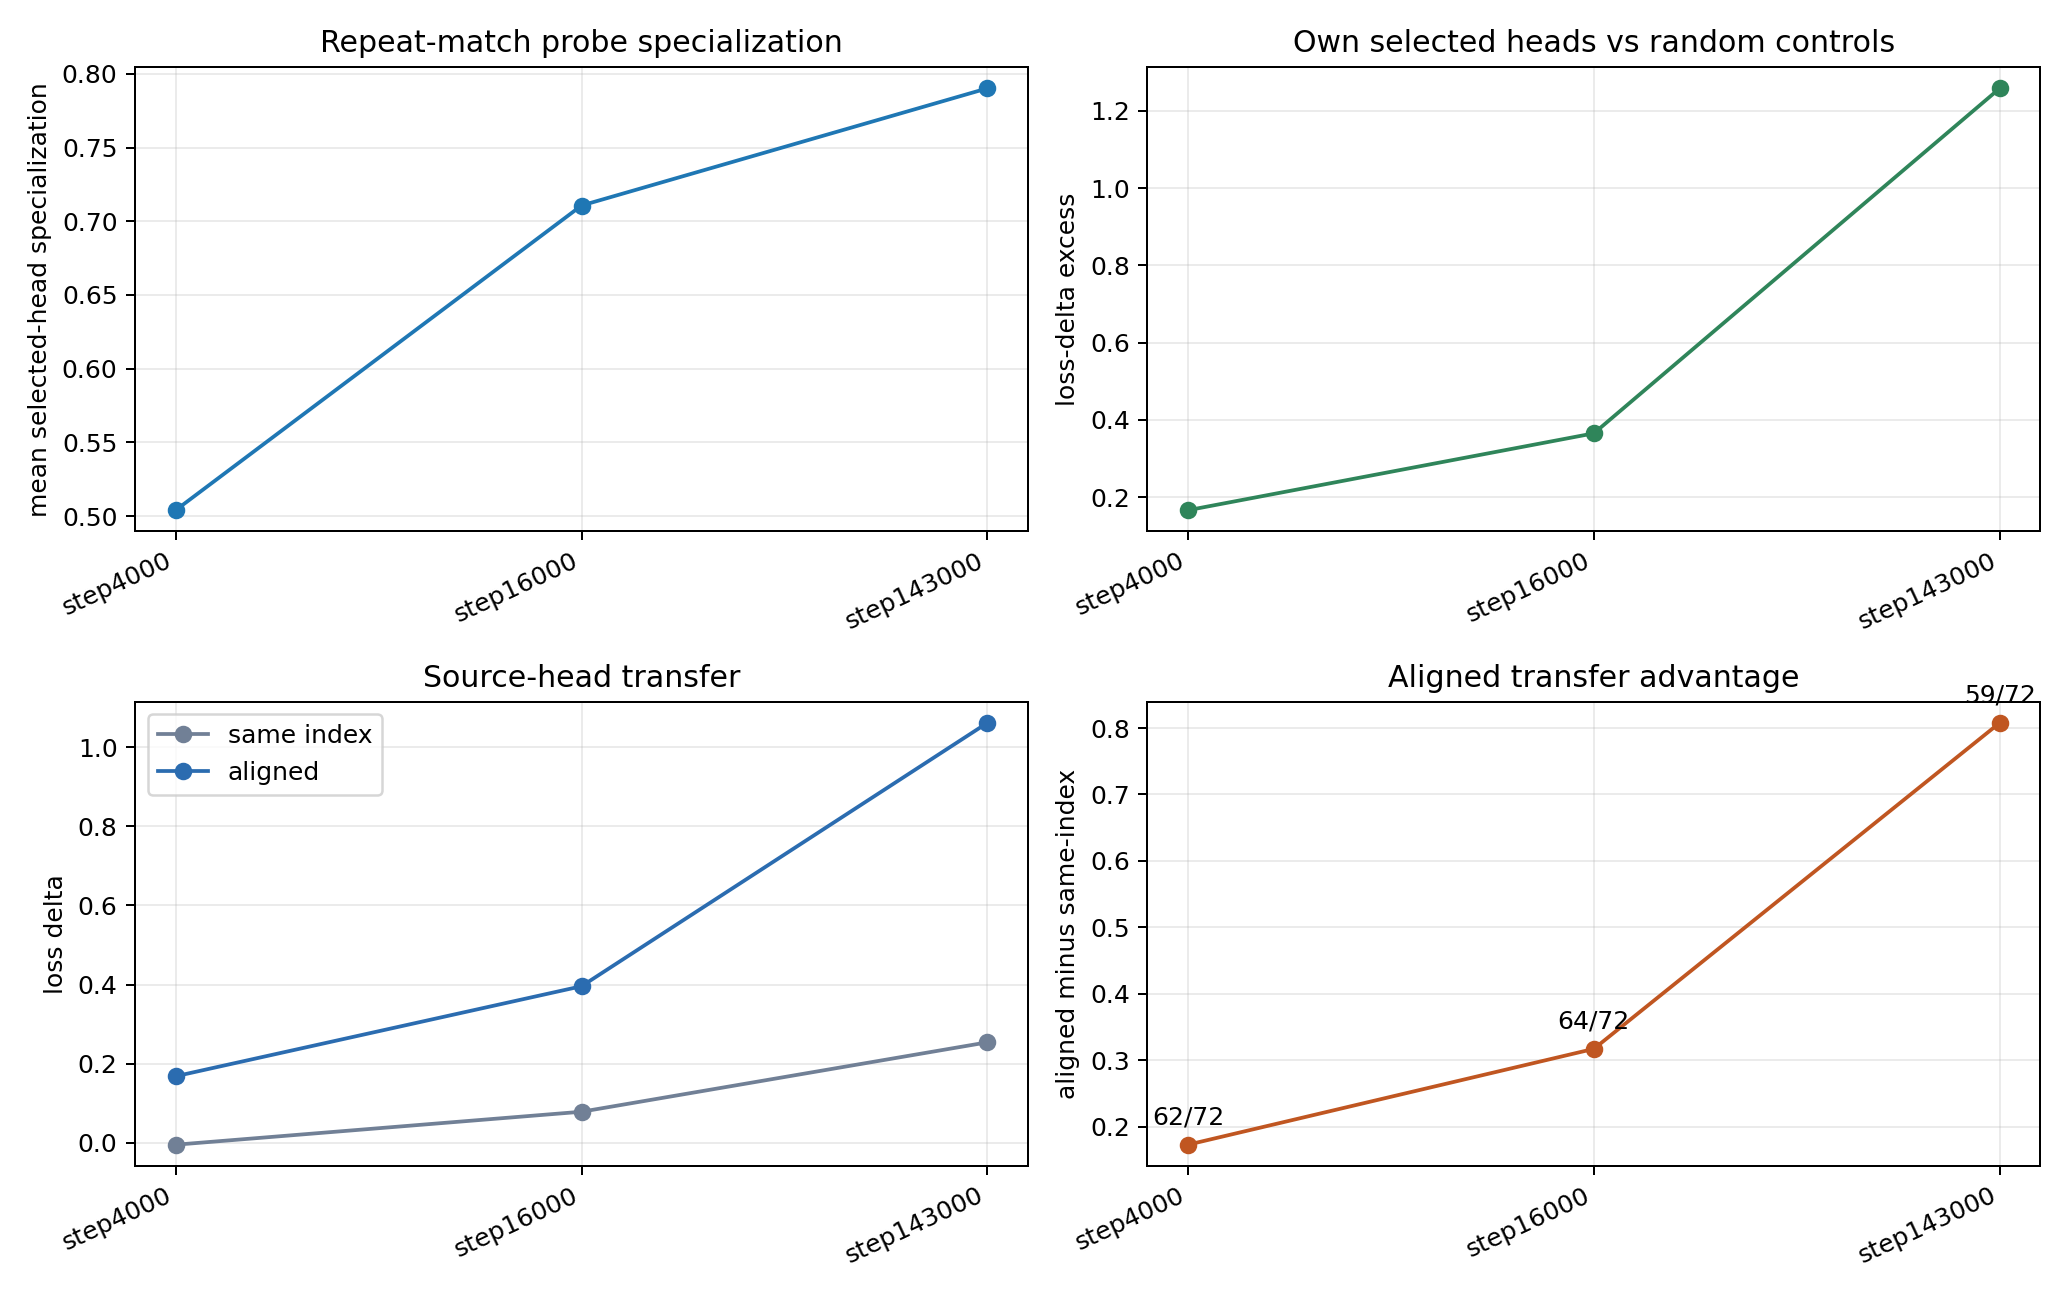
\includegraphics[height=0.70\textheight,keepaspectratio]{../figures/seed9_alignment_selected_trajectory.png}
  \end{center}

  \small
  Alignment transfer is already detectable by step4000 and grows strongly by the
  final checkpoint.
\end{frame}

\begin{frame}{Aggregate Results}
  \scriptsize
  \begin{center}
  \begin{tabular}{lrrrrrr}
    \toprule
    Revision & Probe & Own $-$ rand. & Same-index & Aligned & Align $-$ same & Better \\
    \midrule
    step4000 & 0.5039 & 0.1659 & -0.0049 & 0.1682 & 0.1731 & 62/72 \\
    step16000 & 0.7107 & 0.3650 & 0.0785 & 0.3958 & 0.3173 & 64/72 \\
    step143000 & 0.7903 & 1.2586 & 0.2541 & 1.0619 & 0.8078 & 59/72 \\
    \bottomrule
  \end{tabular}
  \end{center}

  \vspace{0.6em}
  \small
  Means over 9 seeds. Transfer means use 72 ordered source-target seed pairs per
  checkpoint.
\end{frame}

\begin{frame}{What Changed From The 3-Seed Pilot}
  \textbf{Confirmed}
  \begin{itemize}
    \item Raw-score alignment transfers causal repeat-match roles much better
    than raw same-index transfer.
    \item Same-index transfer remains weak at every selected checkpoint.
  \end{itemize}

  \vspace{0.7em}
  \textbf{Revised}
  \begin{itemize}
    \item The 3-seed pilot made step4000 look mostly probe-only.
    \item The 9-seed run shows measurable aligned causal transfer already at
    step4000: aligned-minus-same is 0.1731 and aligned wins in 62/72 pairs.
  \end{itemize}
\end{frame}

\begin{frame}{Interpretation}
  \textbf{Supported}
  \begin{itemize}
    \item Repeat-match role identity is weakly universal across Pythia-160M
    seeds after relabeling by raw-score alignment.
    \item Causal role transfer strengthens through training:
    aligned-minus-same rises from 0.1731 to 0.8078.
    \item Probe specialization, causal importance, and aligned transfer all
    strengthen across training, but not in a clean all-or-nothing sequence.
  \end{itemize}

  \vspace{0.6em}
  \textbf{Not shown}
  \begin{itemize}
    \item This does not prove branch-level functional modularity in ordinary
    Pythia attention heads.
  \end{itemize}
\end{frame}

\begin{frame}{Caveats}
  \begin{itemize}
    \item Only Pythia-160M is covered in the 9-seed scale-up.
    \item Only layers 0 and 1 were tested.
    \item Synthetic repeated-token continuation task.
    \item Head-output zero ablation, not full path patching.
    \item Alignment uses 8 short probe texts; a larger probe corpus remains a
    useful robustness check.
    \item The first all-checkpoint run was interrupted by unrelated GPU
    contention, so the final result uses three completed one-checkpoint jobs.
  \end{itemize}
\end{frame}

\begin{frame}{Decision And Next Step}
  \textbf{Decision.} Treat aligned causal transfer as a validated Phase 1
  metric for repeat-match heads in Pythia-160M.

  \vspace{0.8em}
  \textbf{Next step.}
  Test whether this is specific to repeat-match heads:

  \begin{itemize}
    \item add a second causal head-role task, such as previous-token or
    induction-style copying;
    \item keep same-index transfer as the negative baseline;
    \item add path patching after a second role survives head-output ablation.
  \end{itemize}
\end{frame}

\begin{frame}{Provenance}
  \small
  \textbf{Source}
  \begin{itemize}
    \item \texttt{scripts/pythia\_repeat\_match\_alignment\_trajectory.py}
    \item \texttt{scripts/analyze\_pythia\_alignment\_trajectory.py}
    \item \texttt{scripts/analyze\_pythia\_seed9\_alignment\_selected.py}
    \item \texttt{doc/phase1\_pythia160m\_seed9\_alignment\_selected\_checkpoints.md}
  \end{itemize}

  \vspace{0.4em}
  \textbf{Copied data}
  \begin{itemize}
    \item \texttt{../data/revision\_summary.csv}
    \item \texttt{../data/condition\_summary.csv}
    \item \texttt{../data/transfer\_pair\_summary.csv}
    \item \texttt{../figures/seed9\_alignment\_selected\_trajectory.png}
  \end{itemize}
\end{frame}

\end{document}
